\documentclass[../../master.tex]{subfiles}

\begin{document}
\chapter{Artificial Neural Networks \label{NN}}
The following is a \emph{brief} introduction to the theory underlying the construction and training of artificial neural networks (ANNs). For a more comprehensive review of the subject, the reader is encouraged to survey relevant chapters from the recent master theses of Stende and Treider \cite{stende,treider}. This introduction follows closely the introduction of Raff and co-workers \cite{raff}. 

Artificial neural networks can be created in numerous ways, but we will focus exclusively on the most common architecture, namely \emph{multilayer perceptrons} (MLP). The MLP neural networks are built from \emph{layers} of connected \emph{neurons}. In the artificial network, an input value (possibly a vector) is fed into the network model and then propagated through the layers, being processed through each neuron in turn. We will deal only with \emph{feed forward} ANNs, meaning information always flows through the net in one direction only\textemdash essentially there are no loops. The entire ANN produces an output value (possibly a vector), which means we can think of it as a complicated function $\mathbb{R}^n\mapsto \mathbb{R}^m$. As we will see, it is possible to write down a closed form expression for this function and it is\textemdash crucially\textemdash possible to devise an efficient algorithm for calculating the gradient of the entire function w.r.t.\ any of the internal parameters.

\section{Artifical neurons \label{sneurons}}
A neuron is simply a model function for propagating information through the network. Inspired by biological neurons, the artificial neuron "fires" if it is stimulated by a sufficiently strong signal. The artificial neuron receives a vector of input values ${\bf p}$. If the neuron is part of the very first hidden layer (this will be expanded upon shortly), the input is simply the input value(s) to the NN. If one or more layers preceded the current one, ${\bf p}$ is a vector of outputs from the neurons in the previous layer.


\begin{figure}
\begin{centering}
\begin{tikzpicture}[
node distance = 5mm and 18mm,
  start chain = going below,
  arro/.style = {-Latex},
bloque/.style = {text width=4ex, inner sep=2pt, align=right, on chain},
                        ]
% inputs
\foreach \i [count=\j] in {p_{1}, p_{2}, p_{3}, {\vdots}, p_{N}}
    \node[bloque] (in-\j) {$\i$};
% output
\node (out) [circle, draw, minimum size=6mm,
      %label=\textsc{$\displaystyle\sum_{i=1}^N$},
      right=of $(in-3)!0.5!(in-3)$]  {$\displaystyle\sum_{i=1}^Nw_ip_i$};
% conections
\foreach \i in {1,...,3}
    \draw[arro] (in-\i) -- (out);
\draw[arro] (in-5) -- (out);
% output
\node (output) [circle, draw, minimum size=6mm,right=of out]   
		{$f\left[{\bf w}^T{\bf p} + b\right]$};
%\coordinate[right=of out] (output);
\draw[arro] (out) -- (output);
% layer labels
\node[above=of in-1.center]     {Input};
\node[below=of in-4 -| out]     (bias) [circle,draw,minimum size=6mm]
										{$b$};
\draw[arro] (bias) -- (output);
\node[above=of in-1 -| output]  {Activation};
\node[above=of in-1 -| out]  {Sum};
\node[right=of output] (final) {$\tilde p$};
\node[above=of in-1 -| final]  {Output};
\draw[arro] (output) -- (final);
\end{tikzpicture}
\caption{A model neuron, a constituent part of the artificial neural network model. The input from the previous layer ${\bf p}$ multiplied by corresponding weights ${\bf w}$ and summed. Then the bias $b$ is added, and the activation function $f$ is applied to the resulting ${\bf w}^T{\bf p}+b$. The output $\tilde p$ goes on to become input for neurons in the next layer. \label{fig:neuron}}
\end{centering}
\end{figure}
The neuron is connected to the previous layers' neurons, and the strength of the connection is represented by a vector of weights, ${\bf w}$. Let us now consider a neuron which we will label by the index $k$. The output from neuron $i$ (of the preceding layer), $p_i$, is multiplied by the weight corresponding to the $i$\----$k$ connection, $w_i$. The combined weight vector multiplied by the input vector gives part of the total activation of the neuron, 
\begin{align}
\sum_{i=1}^Nw_ip_i = {\bf w}^T{\bf p}.
\end{align}
The remaining part is known as the bias, $b_k$. This is a single real number. There is one for each neuron, and it acts as modifier making the neuron more or less likely to fire independently of the input. 

The total input is passed to an activation (or transfer) function, which transforms it in some specified way, yielding the neuron \emph{output} $\hat p_k$. This in turn becomes input for the neurons in subsequent layers. 

Various different activation functions $f$ are used for different purposes. The function may be linear or non-linear, but should vanish for small inputs and \emph{saturate} for large inputs. For reasons that will become clear shortly, the conditions we enforce on $f$ is continuity, boundedness, as well as non-constantness. We also demand it be monotonically increasing. A popular example, the sigmoid, takes the form 
\begin{align}
f(x) = \frac{1}{1+\mathrm{e}^{-x}}.
\end{align}
An example of the sigmoid is shown in \fig{sigmoid}. Numerous alternative transfer functions are in popular use, including the hyperbolic tangent $\tanh$, the inverse tangent $\tan^{-1}$, the rectified and exponential linear units (ReLU and ELU), Gaussians, and identity functions $f(x)=x$.

In total, the action of a single neuron can be written
\begin{align}
\text{input}\ \rightarrow f\left({\bf w}^T{\bf p}+b\right) = \tilde p \ \rightarrow \ \text{output}.
\end{align}
A schematic representation of the single neuron connected to the previous and acting as input for the next layers is shown in \fig{neuron}. 

\begin{SCfigure}
\centering
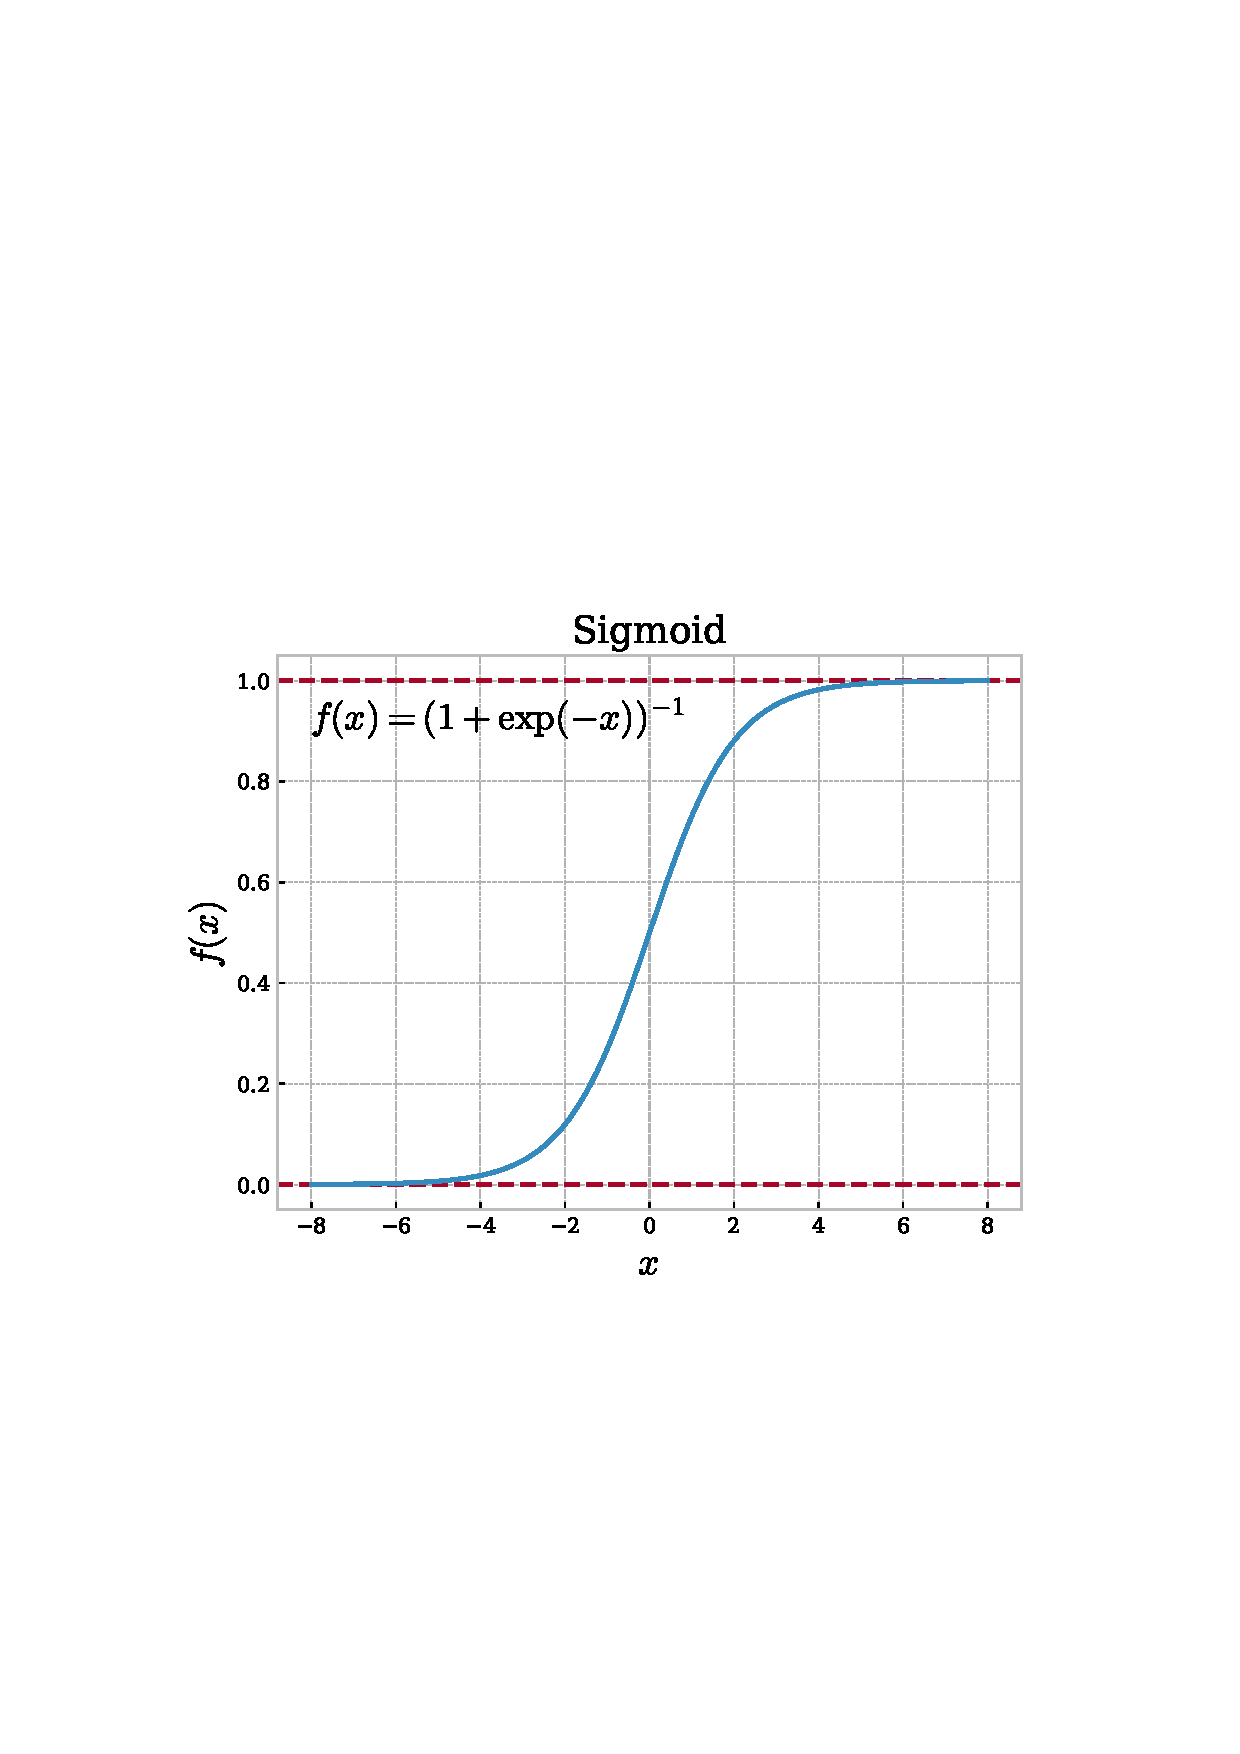
\includegraphics[width=0.49\textwidth, trim=0 200 0 200, clip]{sigmoid.pdf}
\caption{Example of a \emph{sigmoid} function, used as a non-linear activation function for artificial neural networks.\label{fig:sigmoid}}
\end{SCfigure}

\section{Network layers}
The full artificial neural network is built up of layers of neurons. Data is fed sequentially through the network, starting in the input layer (the input values can be thought of as the first layer), through the \emph{hidden} layers, and ending up in the output layer. The propagation needs to happen simultaneously across the network, as layer $k$ needs the fully computed output of layer $k-1$ before the activations can be calculated. 

\renewcommand{\b}{{\bf b}}
\newcommand{\y}{{\bf y}}
A layer is\textemdash put simply\textemdash a collection of neurons, all of which are connected to the previous layer's neurons and the next layer's neurons. Let us label the individual neurons in layer $k$ by index $i$, i.e.\ $n_i^k$. The bias of neuron $i$ is then denoted $b^k_i$, and the weights connecting $n_i^{k-1}$ to $n_j^k$ is called $w_{ji}$. For each neuron there is a corresponding weight, so the weight vector is denoted $\bm{w}_i^k$. The combination of all weight vectors for layer $k$ thus makes a matrix, which we will denote by a capital $W^k$,
\begin{align}
W^k=\pmat{ccccc}{
	w^k_{11} & w^k_{12} & w^k_{13} & \dots & w^k_{1N} \\
	w^k_{21} & w^k_{22} & w^k_{23} & \dots & w^k_{2N} \\
	w^k_{31} & w^k_{32} & w^k_{33} & \dots & w^k_{3N} \\
	\vdots  &  \vdots   &   \vdots   & \ddots & \vdots \\
	w^k_{N1} & w^k_{N2} & w^k_{N3} & \dots & w^k_{NN}
}, 
\end{align}
or more compactly $(W^k)_{ij}=w^k_{ij}$. The collection of all biases for layer $k$ is $\b^k$. In this notation, we may write the propagation of the signal from layer $k-1$ to layer $k$ as 
\begin{align}
\y^k &= f(W^k\y^{k-1}+\b^k) \nn\\ 
&=f\left( \bmat{ccccc}{
	w^k_{11} & w^k_{12}  & \dots & w^k_{1N} \\
	w^k_{21} & w^k_{22}  & \dots & w^k_{2N} \\
	\vdots  &  \vdots      & \ddots & \vdots \\
	w^k_{N1} & w^k_{N2}  & \dots & w^k_{NN}
} 
 \bmat{c}{y^{k-1}_1\\ y^{k-1}_2  \\ \vdots \\ y^{k-1}_N}  
+\bmat{c}{b^{k}_1  \\ b^{k}_2    \\ \vdots \\ y^{k}_N} \right) \label{eq:nnmatrix}
\end{align}
or in Einstein notation 
\begin{align}
y^k_i= f\big(w^k_{ij}y^{k-1}_j+b^k_i  \big). \ \ \ \ \ \ \ \ \ (\text{no sum over }k\text{ implied})
\end{align}
In all of the preceeding three equations, application of $f$ indicates \emph{element wise} functional evaluation.

It is clear from \eq{nnmatrix} that propagation through an entire layer can be thought of as a matrix-vector product, a vector-vector summation, and a subsequent application of the transfer function $f$ element-wise on the resulting vector. 

A schematic representation of a layer consisting of three artificial neurons in a fully connected ANN is shown in \fig{layer}.

%Raff s. 51: "NN (and other non-linear black box techniques) cannot be expected to \emph{extrapolate} accurately."

\begin{SCfigure}
\begin{centering}
\def\layersep{2.5cm}
\begin{tikzpicture}[shorten >=1pt,->,draw=black!50, node distance=\layersep]
    \tikzstyle{every pin edge}=[<-,shorten <=1pt]
    \tikzstyle{neuron}=[circle,minimum size=17pt,inner sep=0pt]
    \tikzstyle{input neuron} =[neuron, draw=gray];
    \tikzstyle{output neuron}=[neuron, draw=gray];
    \tikzstyle{hidden neuron}=[neuron, fill=black];
    \tikzstyle{annot} = [text width=4em, text centered]

    % Draw the input layer nodes
    \foreach \name / \y in {1,...,3}
    % This is the same as writing \foreach \name / \y in {1/1,2/2,3/3,4/4}
        \node[input neuron, pin=left:{}] (I-\name) at (0,-\y) {};

    % Draw the hidden layer nodes
    \foreach \name / \y in {1,...,3}
        \path[yshift=0.0cm]
            node[hidden neuron] (H-\name) at (\layersep,-\y cm) {};

    % Draw the output layer node
	%\foreach \name / \y in {1,...,3}
    %    \path[yshift=0.0cm]
    %        node[hidden neuron] (H-\name) at (-\layersep,-\y cm) {};
   	\node[output neuron,pin={[pin edge={->}]right:{}}, right of=H-3] (O) {};
   	\node[output neuron,pin={[pin edge={->}]right:{}}, right of=H-3] at (\layersep,-1) (OO) {};
   	\node[output neuron,pin={[pin edge={->}]right:{}}, right of=H-3] at (\layersep,-2) (OOO) {};

   	
    % Connect every node in the input layer with every node in the
    % hidden layer.
    \foreach \source in {1,...,3}
        \foreach \dest in {1,...,3} 
            \path (I-\source) edge (H-\dest);
            

    % Connect every node in the hidden layer with the output layer
    \foreach \source in {1,...,3} {
        \path (H-\source) edge (O);
		\path (H-\source) edge (OO);
		\path (H-\source) edge (OOO);
		}

    % Annotate the layers
    \node[annot,above of=H-1, node distance=1cm] (hl) {Layer\ \ \ \ \ $k$};
    \node[annot,left of=hl]  {Layer\ \ \ $k-1$};
    \node[annot,right of=hl] {Layer\ \ \ $k+1$};
\end{tikzpicture}
\end{centering}
\caption{Schematic representation of a single ANN layer. Each neuron of the layer indexed $k$ is connected from behind to all neurons in layer $k-1$. The connection weights can be organized into a matrix, $W^{k-1}$, and the action of layer $k$ can be succinctly stated as $f(W^{k}{\bf p}^{k-1}+{\bf b}^k)$ where element-wise operation is assumed for the activation $f$. \label{fig:layer}}
\end{SCfigure}

\section{The full network}
A collection of $L$ layers connected to eachother forms a full \emph{network}. Note carefully that the network is nothing more than a (somewhat complex) function. If a single input and a single output value is specified, the action of the NN can be written out in closed form as \cite{stende}
\begin{align}
&\hat y\! = \!\left.\!\sum_{j=1}^{M}\! w_{1j}^L f\!\left(\!\sum_{k=1}^{M}\! w_{jk}^{L-1} f\!\left(\!
\sum_{i=1}^Mw_{ki}^{L-2} f\left( \dots \!f\!\Big(\!w_{m1}^1 x_1 \! + \!b_m^1\!\Big)
 \!\dots \!\right)+ b_i^{L-2}\right) \!+ \!b_k^{L-1}\!\right)
 \!+ \!b_1^L\!\right. && \label{eq:nnfull}
\end{align}
Here, we have taken the each layer to consist of $M$ neurons. The scalar $x_1$ denotes the input value, while $\hat y$ is the NN output. From looking at \eq{nnfull}, the usefulness of the model is in no way obvious. But it turns out that for an ANN with at least one hidden layer populated with a finite amount number of neurons is a \emph{universal approximator} \cite{HORNIK1989359}. This holds under the aforementioned assumptions on $f$, c.f.\ section \ref{sneurons}. Being a universal approximator means (in this context) that the NN function can be made to be arbitrarily close to any continuous Borel-measurable function (essentially \emph{any} function we are likely to encounter) \cite{mcdonald}. 

\section{Training the ANN}
Knowing that ANNs can be universal approximators is not helpful unless we can find a systematic way of obtaining suitable parameters to approximate any given function $g(x)$. This is where \emph{training} comes in. In section \ref{AI} we defined machine learning as the science of creating computers capable of learning from experience. Teaching a NN to approximate a function is conceptually simple, and involves only three steps:
\begin{shadeframe}
Assume input $x$ and corresponding \emph{correct} output $y$ is known.
\begin{itemize}
	\item[(1)] Compute output $\text{NN}(x)=\hat y$ of the artificial neural network, and evaluate the \emph{cost} function, typically $C(\hat y)\equiv \Vert y-\hat y\Vert_2$. 
	\item[(2)] Compute the gradient of $C(\hat y)$ w.r.t.\ all the parameters of the network, $w_{ij}^k$ and $b^k_j$.  
	\item[(3)] Adjust the parameters according to the gradients, yielding a better estimate $\hat y$ of the true output value $y$. 
	\item[(4)] Repeat (1)\textemdash(4).
\end{itemize}
\end{shadeframe}
The training scheme is known as \emph{supervised learning}, because the NN is continually presented with $x$, $y$ pairs, i.e.\ an input and an expected output. The cost (or objective or loss) function determines how happy the network is with it's own performance. A common choice for the cost function is the $\ell^2$ norm, essentially the root squared difference,
\begin{align}
C(\hat \y) = \Vert \y-\hat \y\Vert_2= \sqrt{\sum_{i=1}^{N_\text{O}}(y_i-\hat y_i)^2}. \label{eq:cost}
\end{align}
In general, the output of the neural network is a vector of values, $\y$, and the cost function is taken across all outputs. In \eq{cost}, the network produces $N_\text{O}$ outputs for each input (which itself may be a vector). 

Step (3) is easy to understand, but complex in practice. In order to update the network weights and biases, a measure of the expected change in the total output is needed. Otherwise, any change would just be done at random\footnote{This is a possible approach, yielding a class of \emph{genetic} optimization algorithms. We will not discuss such schemes in the present work.}. This means we need to compute the set of derivatives 
\begin{align}
g_{ij}^k \equiv \pder{C(\hat \y)}{w_{ij}^k}, \ \ \ \text{ and } \ \ \ h_i^k\equiv \pder{C(\hat \y)}{b^k_i}.
\end{align}
The most common algorithm for computing these derivatives is the {\bf backpropagation} algorithm \cite{backprop}. The method works by first pushing an input through the ANN, and computing the derivatives of the cost function w.r.t.\ the last layer weights and biases. The network is then traversed backwards, and the gradient w.r.t.\ all neuron parameters is found by repeated application of the chain rule. An explicit statement of the algorithm is found in any book on neural networks, see e.g.\ Raff and co-workers \cite{raff}.

The final step in the training algorithm constitutes updating the weights according to the computed gradient. Possibly the simplest scheme for updating the weights is to just blindly follow the direction of the negative gradient, moving some set step length $\mathit{\Delta}w$ and $\mathit{\Delta}b$. This is known as \emph{gradient descent}, or \emph{steepest descent}. Since the gradient represents the direction in the parameter-hyperspace giving the fastest decrease in $C(\hat \y)$, this will in principle lead to a minimum. However, modern ANN methods use more sophisticated optimization schemes. 

Whereas the gradient descent is a \emph{first order} optimization algorithm\textemdash depending only on the first derivative (gradient)\textemdash it is possible to devise higher order methods taking advantage of the information contained in e.g.\ the second derivative (Hessian matrix). Often, the second order schemes require calculation and inversion of the Hessian. This is true of for example Newton's method, which minimizes $C(\hat \y)$ by finding the roots of 
\begin{align}
\nabla C(\hat \y)=0. 
\end{align}
If the Hessian is too expensive to compute directly, it may be possible to estimate it in a computationally more feasible manner. This leads to a class of optimization algorithms known as Quasi-Newton methods, see e.g.\ the algorithm of Barzilai and Borwein \cite{BARZILAIBORWEIN}.

A popular approach in modern ANN codes is using gradient descent based methods which automaticall adjust the training rate (the stepping size) for each parameter individually. The Adagrad and Adadelta methods are both examples of such methods, which also attempt to fine-tune the learning rate by considering a decaying backlog of stored squared gradient values \cite{opti}. The algorithm we will use in the present work is called Adam (derived from [but not an acronym for] \emph{adaptive moment estimation}), which stores exponentially decaying averages of both gradients and squared gradients in order to find optimal step sizes \cite{adam}. For an accessible introduction to the specifics of the Adam optimizer, see e.g.\ the recent Master thesis of Stende \cite{stende}.


















































\end{document}